\chapter{Experiments and Results}
\label{ch:results}

This chapter presents the measured results. For each result three things are stated:
the observed value, the denominator and measurement conditions, and the ``permitted
claim boundary'' based on its evidence class (Table~\ref{tab:evidence-classes}). All
numbers in this chapter are read from the project's recorded and hashed artifacts, and
none is an estimate.

\section{Coverage of Acceptance Conditions and Evidence Status}
\label{sec:res-gates}

Table~\ref{tab:gates} places the status of the project's ``official'' acceptance
conditions, as produced by the fail-closed aggregator, next to the automatic evidence of
the final stage. The official conditions are deliberately strict (human labels, physical
target hardware, a complete human study) and the automatic evidence does not replace
them; the third column shows how far each condition is covered by automatic evidence.

\begin{table}[ht]
\centering
\caption{The project's official acceptance conditions and the automatic evidence of the
         final stage}
\label{tab:gates}
\small
\begin{tabular}{L{5.0cm}cL{5.2cm}}
\toprule
\textbf{Acceptance condition} & \textbf{Official status} & \textbf{Final automatic evidence} \\
\midrule
Working Persian speech-to-speech prototype & sufficient & streaming system, browser loopback test \\
Passing the final automatic semantic test & sufficient & -- \\
Audited export within 100--200 hours & sufficient & -- \\
Data policy resolved under a documented review waiver & sufficient & -- \\
Source code licence chosen & sufficient & -- \\
\midrule
Deployable direct Persian model & negative & Moshi v7a: 6/9, unintelligible speech; Gemma speech input: negative \\
Detector with accuracy above 80\% on independent labels & not human &
  simulation 0.933/0.880; browser 0.825/0.817 \\
Fit and live latency on 12--24 GB hardware & not target hardware &
  memory 11.1~GiB; mean 372 and 90th percentile 431 ms on an H100 \\
Completion of the human study & pending & registered instrument and protocol; responses not yet received \\
\bottomrule
\end{tabular}
\end{table}

\claim{Five engineering conditions have sufficient official evidence. For the three
conditions of the detector, latency and memory, the automatic evidence meets the
numeric criteria of the proposal, but with automatic labels and on an H100; the direct
model is negative and the results of the human study are not yet available.}

\section{Dataset}
\label{sec:res-data}

Table~\ref{tab:corpus} shows the final characteristics of the dataset.

\begin{table}[ht]
\centering
\caption{Characteristics of the derived Persian conversational dataset and its
         automatic audit}
\label{tab:corpus}
\small
\begin{tabular}{L{7.6cm}R{3.4cm}}
\toprule
\textbf{Indicator} & \textbf{Value} \\
\midrule
Caption inventory of the channels & 775.887 hours \\
Long programmes in the inventory & 1,442 \\
Selected programmes & 309 \\
Candidate windows & 1,129 \\
Candidate hours after selection & 219.946 hours \\
Automatically classified multi-speaker hours & 207.154 hours \\
\midrule
Response pairs without reuse & 6,754 \\
Source audio hours of the pairs & 123.796 hours \\
Speakers & 407 \\
Sessions & 162 \\
\midrule
Exported stereo pairs & 6,754 \\
Exported stereo hours & 108.584 hours \\
Train / validation / test split & 6,419/131/204 \\
Group leakage & 0 \\
Missing files in the audit & 0 \\
Automatic audit failures & 0 \\
\midrule
Automatic interaction-event candidates & 770 \\
of which interruption-like / backchannel-like & 717/53 \\
Human-verified rows & 0 \\
\bottomrule
\end{tabular}
\end{table}

The 108.584 hours lie within the 100--200 hours of requirement R4, and the automatic
integrity audit, including checks of channel order, file hashes and group splits, passed
without failure.

\textbf{Independent verification of the labels.} The turn-boundary and overlap labels
were measured with an independent automatic listener (Gemini~3.8~Flash, two prompts with
different wording and agreed labels only) on 300 pairs of the second balanced version;
the sample was drawn from the 1,353 pairs whose source audio was still on disk after the
audio was moved to cloud backup (mostly two of the four channels). At 93.8\% of turn
boundaries, the independent listener heard another speaker start (two-level confidence
intervals of about 87--97\%). The marked overlaps were heard as overlaps in 75.7\% of
cases, but the listener also heard overlap at a third of the unmarked boundaries; that
is, diarization under-reports short overlaps. The turn captions differ from the
listener's verbatim transcript by a character error rate of 15.9\%. The agreement of the
two prompts was 71--73\%.

\claim{This result is an \emph{automatic} audited export. The interaction labels are
automatic candidates and the number of human-verified rows is zero; this dataset can
therefore not be called ``human-labelled''; the verification above is also automatic and
was run on an available sample. The source data are not redistributable.}

\section{Cascade System: Mechanical Panel}
\label{sec:res-cascade}

The validation panel is nine evenly spaced rows of the 131-row validation manifest. The
indices of these rows were locked before running. The chain run is the real speech
recognition service, the local Qwen2.5-0.5B-Instruct responder and the real speech
engine, and the input channel is the audited user channel one. This panel measures the
mechanics of the chain, not the semantic quality of the Qwen3-4B responder of the
delivered system. The aggregate result of the panel is in Table~\ref{tab:cascade-panel}.

\begin{table}[ht]
\centering
\caption{Result of the fixed validation panel of the cascade}
\label{tab:cascade-panel}
\small
\begin{tabular}{L{7.6cm}R{3.4cm}}
\toprule
\textbf{Indicator} & \textbf{Value} \\
\midrule
Rows of the validation manifest & 131 \\
Split unit & source session identifier \\
Split leakage & 0 \\
Predefined evaluated rows & 9 \\
Text responder of the panel & Qwen2.5-0.5B-Instruct \\
\midrule
Rows passing every condition & 9/9 \\
Rows with a rule-based fallback reply & 0/9 \\
Rows with a language retry & 0/9 \\
Recognition service errors & 0 \\
Language model load or generation failures & 0/9 \\
Minimum Persian-character share in the transcript & 1.000 \\
Minimum Persian-character share in the reply & 1.000 \\
Non-silent audio replies & 9/9 \\
Minimum RMS of the reply audio & 0.133529 \\
Final-test rows used & 0 \\
\bottomrule
\end{tabular}
\end{table}

Table~\ref{tab:cascade-rows} gives the details of each row. The time column is the
duration of ``full reply generation'', not the latency of the first audio.

\begin{table}[ht]
\centering
\caption{Measurements of each row of the cascade validation panel}
\label{tab:cascade-rows}
\small
\begin{tabular}{rrrrrc}
\toprule
\textbf{Manifest} & \textbf{Transcript} & \textbf{Reply audio} &
\textbf{RMS} & \textbf{Full generation} & \textbf{Pass} \\
\textbf{row} & \textbf{characters} & \textbf{duration (s)} &
 & \textbf{time (ms)} & \\
\midrule
0   & 35   & 4.644 & 0.184925 & 4895.3  & yes \\
16  & 541  & 5.352 & 0.162841 & 5473.7  & yes \\
32  & 5031 & 7.535 & 0.210650 & 13270.2 & yes \\
48  & 1237 & 9.857 & 0.191641 & 7414.3  & yes \\
65  & 445  & 9.288 & 0.162643 & 6664.3  & yes \\
81  & 2398 & 7.465 & 0.133529 & 12709.4 & yes \\
97  & 77   & 3.448 & 0.193290 & 2072.4  & yes \\
113 & 405  & 5.259 & 0.191777 & 3674.2  & yes \\
130 & 142  & 8.824 & 0.154569 & 5584.7  & yes \\
\bottomrule
\end{tabular}
\end{table}

A retrospective, privacy-preserving descriptive analysis was also run on the same report;
it reads only aggregate values and hashes and does not read or publish transcript or reply
text. Its findings are: no mechanical failure occurred; the median, 95th percentile and
maximum transcript lengths were 445, 3977.8 and 5031 characters; the median, 95th
percentile and maximum full generation times were 5584.736, 13045.919 and 13270.249 ms;
three rows had transcripts of more than 1000 characters and two rows generation times of
more than 10 seconds.

The most important engineering risk observed is the growth of full generation time with
input length. The descriptive Pearson correlation between transcript length and full
generation time is 0.885, and the longest transcript and the slowest turn were both row 32.
Figure~\ref{fig:cascade}(a) shows this relationship.

\begin{figure}[ht]
\centering
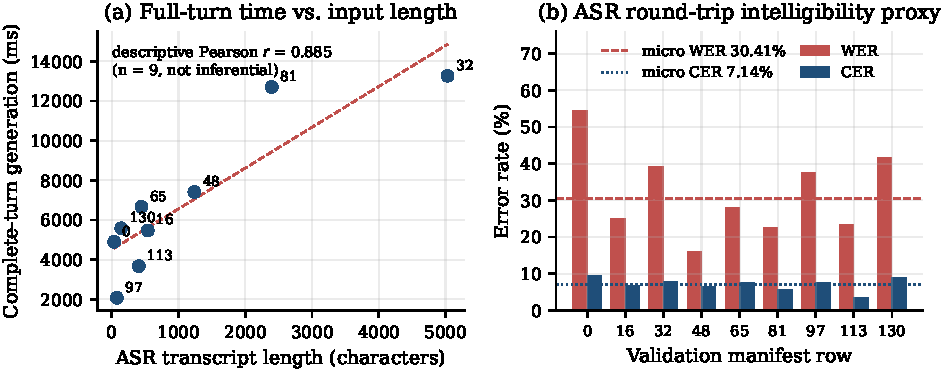
\includegraphics[width=\textwidth]{figs/cascade_panel.pdf}
\caption{(a) Full reply generation time against input transcript length for the nine
         rows of the validation panel, with the fitted line and the descriptive Pearson
         correlation. (b) Word and character error rates of re-recognition for the same
         nine outputs, with the micro-aggregated values.}
\label{fig:cascade}
\end{figure}

\claim{This is a positive mechanical, out-of-sample result on a group-disjoint panel
with the Qwen2.5-0.5B responder. A nine-row panel is not enough to prove population
generalization or semantic quality and is not generalized to the Qwen3-4B responder of
the delivered system. The reported correlation is descriptive, not inferential. Full
generation time on the available hardware is not the $T_{\text{first\_audio}}$ measure
and cannot meet the 500 ms condition.}

\section{Automatic Approximation of the Intelligibility of Generated Speech}
\label{sec:res-intel}

To measure whether the generated speech preserves the content of the reply text, a
re-recognition measurement was run on the same nine outputs of the chain with the
Qwen2.5-0.5B responder: the generated reply text is the reference and the recognition
service's transcript of the output waveform the hypothesis. The protocol of this
measurement, including normalization, token definitions and validity conditions, was
registered before running, and all input hashes were reproduced. The result is reported
in Table~\ref{tab:intel}.

\begin{table}[ht]
\centering
\caption{Result of the automatic re-recognition approximation of the generated speech}
\label{tab:intel}
\small
\begin{tabular}{L{6.8cm}R{4.0cm}}
\toprule
\textbf{Indicator} & \textbf{Value} \\
\midrule
Valid rows / recognition service errors & 9/0 \\
\midrule
Reference words / word edits & 171/52 \\
Micro-aggregated word error rate & 30.41\% \\
Macro-averaged word error rate & 32.01\% \\
Word error rate, median / 95th percentile / maximum & 28.00\%/49.40\%/54.55\% \\
\midrule
Reference characters / character edits & 658/47 \\
Micro-aggregated character error rate & 7.14\% \\
Macro-averaged character error rate & 7.13\% \\
Character error rate, median / 95th percentile / maximum & 7.50\%/9.40\%/9.62\% \\
\midrule
Rows with an exact word match & 0/9 \\
Rows with an exact character match & 0/9 \\
\bottomrule
\end{tabular}
\end{table}

Figure~\ref{fig:cascade}(b) shows the distribution of these two error rates row by row.
The striking gap between the character error rate and the word error rate is
interpreted in Section~\ref{sec:disc-cer-wer}.

\claim{This measure is an automatic approximation of ``content preservation'' with a
single voice, on the output of the Qwen2.5-0.5B responder. Because the recognition
service takes part both in the system and in the measurement, and because nine outputs
are not enough to estimate a confidence interval, this result does not prove human
intelligibility, correct pronunciation, naturalness or semantic quality and is not
generalized to the Qwen3-4B responder. No pass threshold was set after seeing the
result.}

\section{Automatic Semantic Test}
\label{sec:res-semantic}

\subsection{Qualification Stage}

The design of this evaluation has two stages. The first stage ran on seven previously
unused validation rows and passed every condition: all 42 judge calls were valid, the
candidate's mean relevance was 3.857 against 1.000 for the baseline, a relevance gain of
2.857, a mean coherence of 3.571 with a gain of +2.286, a paired win rate of 85.7\% (6/7)
and a rate of relevance of at least two of 100\%. Only after this complete pass was the
final test opened, \emph{once}.

\subsection{Final Test}

The final test ran on 40 rows of the 204-row test manifest, from five held-out source
sessions. Three arms were given to the judge double-blind and in randomized order: the
locked Qwen2.5-0.5B baseline, the Qwen3-4B candidate with prompt v2, and the
automatically aligned reference turn of the next speaker. The judge was Qwen3.8-27B-FP8
at revision 017b9c7af6b5689d5dd426a76e0bc077eb5ca20a, at temperature zero with two
repetitions per row. Each arm and each row received two judge calls for relevance and
coherence. Table~\ref{tab:semantic} shows the result of this test.

\begin{table}[ht]
\centering
\caption{Result of the final automatic semantic test on 40 group-disjoint rows}
\label{tab:semantic}
\small
\begin{tabular}{L{6.6cm}R{4.4cm}}
\toprule
\textbf{Indicator} & \textbf{Value} \\
\midrule
Test rows & 40 \\
Source sessions & 5 \\
Valid / expected judge calls & 240/240 \\
Failed judge calls & 0 \\
Judge repetition agreement & 1.00 \\
\midrule
Candidate mean relevance & 3.150 \\
Baseline mean relevance & 1.425 \\
Aligned reference mean relevance & 0.950 \\
Candidate mean coherence & 3.325 \\
Baseline mean coherence & 1.525 \\
\midrule
Relevance gain over the baseline & +1.725 \\
Coherence gain over the baseline & +1.800 \\
Paired relevance wins & 27/40 (67.5\%) \\
Relevance of at least two & 35/40 (87.5\%) \\
\midrule
Candidate generation retries & 0 \\
Invalid candidate audio & 0 \\
\bottomrule
\end{tabular}
\end{table}

Table~\ref{tab:semantic-gates} shows that all seven predefined automatic conditions are
met. No threshold changed after seeing the result.

\begin{table}[ht]
\centering
\caption{Predefined automatic conditions of the final test and the observed values}
\label{tab:semantic-gates}
\small
\begin{tabular}{L{5.8cm}rrc}
\toprule
\textbf{Condition} & \textbf{Threshold} & \textbf{Observed} & \textbf{Status} \\
\midrule
Candidate mean relevance & $\ge$ 2.00 & 3.150 & met \\
Candidate mean coherence & $\ge$ 2.50 & 3.325 & met \\
Relevance gain & $\ge$ 0.50 & 1.725 & met \\
Coherence gain & $\ge$ 0 & 1.800 & met \\
Paired relevance win rate & $\ge$ 0.60 & 0.675 & met \\
Rate of relevance at least two & $\ge$ 0.70 & 0.875 & met \\
Full mechanical validity & 240/240 & 240/240 & met \\
\bottomrule
\end{tabular}
\end{table}

\claim{Passing seven automatic conditions does not mean perceptual quality or an
independent benchmark. The judge and the candidate are of the same family, and this result
stays in the class of automatic approximation.}

Figure~\ref{fig:semantic} shows the mean score of each arm and the full distribution of
scores. A notable point in part (b) is the bimodal distribution of the baseline: the
0.5-billion-parameter model received the full score on some rows and zero on a larger
share. The automatically aligned reference arm also has the lowest score; this observation
is interpreted in Section~\ref{sec:disc-reference}.

\begin{figure}[ht]
\centering
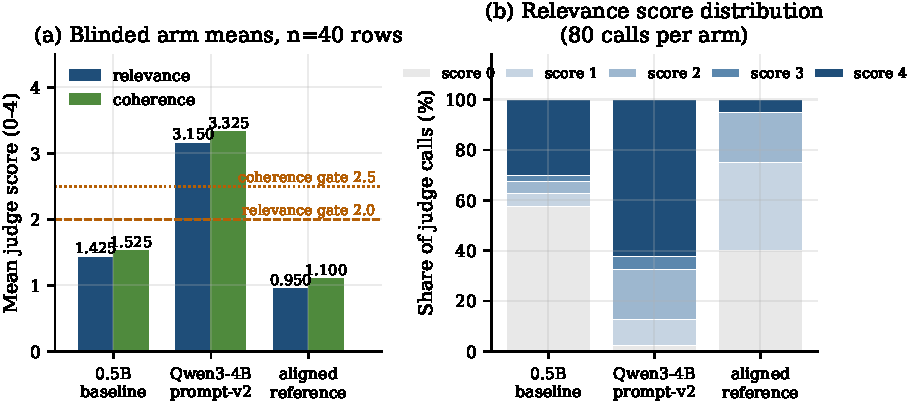
\includegraphics[width=\textwidth]{figs/semantic_final_test.pdf}
\caption{(a) Mean relevance and coherence scores of the three blind arms, with the
         predefined thresholds. (b) Full distribution of the relevance score over the 80
         judge calls of each arm.}
\label{fig:semantic}
\end{figure}

\claim{This is a positive \emph{automatic} result judged by a language model of the
candidate's family. It does not prove human evaluation, an independent dialogue
benchmark, factuality or safety, naturalness, population generalization, target-hardware
fit or browser latency.}

\subsection{Responder Adaptation with LoRA}
\label{sec:res-lora}

A side experiment examined whether low-rank adaptation of the text responder on the
response turns of this dataset improves semantic quality. Training ran successfully and
the development loss decreased: the response-token loss of the base model was 3.723, after
the first epoch 2.643 and after the second 2.562, that is, a 31.18\% reduction relative to
the base model. The second-epoch checkpoint was selected on the lowest development loss.

But semantic evaluation on the forty test rows showed that this adapter does not beat the
baseline. The result was recorded as a ``valid negative result'' and the adapter was not
used in the final system. The interpretation of this apparent contradiction is in
Section~\ref{sec:disc-reference}.

\section{Re-Selection of Components on Fresh Panels}
\label{sec:reselection}

The final audit showed that the earlier speech recognition panels were no longer
independent (newer versions of the recognition models had been trained on the same
YouTube channels), the responder judge was of the candidates' family, and the voice had
never been measured with more than one automatic listener. All three components were
compared again under new, pre-registered protocols.

\subsection{Speech Recognition on Human Transcripts}

The reference of this comparison is the public PSRB benchmark: 344 clips with human
transcripts from various sources (47 clips of older speakers and 183 noisy, telephone or
reverberant clips) on which none of the candidates was trained. Scoring used a
normalizer without punctuation. Latency is the time for a single clip on an H100, and the
latency budget of the streaming system was set to 150 ms (Table~\ref{tab:asr-v2}).

\begin{table}[ht]
\centering
\caption{Comparison of speech recognition candidates on 344 PSRB clips with human
         transcripts}
\label{tab:asr-v2}
\small
\begin{tabular}{lrrrr}
\toprule
Candidate & CER & WER & CER (senior) & Median latency \\
\midrule
NeMo v4 CTC (deployed) & 9.44\% & 23.95\% & 15.63\% & 58 ms \\
NeMo v6 CTC & 10.15\% & 24.34\% & 16.36\% & 60 ms \\
NeMo v4 RNNT & 13.40\% & 26.81\% & 22.10\% & 61 ms \\
omniASR CTC 1B & 14.04\% & 36.38\% & 14.87\% & 56 ms \\
Seamless v5 fine-tune (accuracy reference) & \textbf{6.92\%} & \textbf{21.03\%} & \textbf{10.38\%} & 671 ms \\
Seamless v6 (step 55000) & 8.99\% & 23.28\% & 10.44\% & 855 ms \\
Qwen3-ASR 1.7B & 20.47\% & 49.46\% & 24.97\% & 1466 ms \\
Gemma 4 E4B (audio input) & 21.04\% & 42.67\% & 26.16\% & 2632 ms \\
Whisper large-v3 & 23.02\% & 47.31\% & 25.46\% & 1101 ms \\
\midrule
\multicolumn{5}{l}{\emph{Second round (v3): Persian checkpoints not compared before}} \\
Shenava Koochik (NeMo CTC) & 8.95\% & 35.34\% & 14.50\% & 65 ms \\
BuzzASR (Whisper fine-tune) & 15.76\% & 36.92\% & 19.99\% & 579 ms \\
Rade-ASR-CTC-3B & 16.11\% & 37.33\% & 30.04\% & 122 ms \\
NVIDIA Persian FastConformer & 19.22\% & 45.54\% & 26.43\% & 69 ms \\
Whisper large-v3-turbo, Persian & 20.22\% & 39.21\% & 22.25\% & 484 ms \\
Whisper large-v3, Persian v4 & 21.54\% & 41.86\% & 24.51\% & 1427 ms \\
Whisper base, Persian & 23.30\% & 49.14\% & 28.21\% & 1027 ms \\
NeuraSpeech 900h & 25.42\% & 48.73\% & 37.42\% & 79 ms \\
\bottomrule
\end{tabular}
\end{table}

Seamless is the most accurate candidate but takes more than four times the latency
budget; among the candidates within the budget, NeMo version 4 with a CTC decoder has the
lowest error and stayed in the system. Seamless was used as the ``second independent
listener'' in measuring speech intelligibility and in selecting backchannels. The error
of every candidate is higher on older speakers (15.6\% against 8.6\% for the deployed
candidate).

A second, pre-registered round added the eight Persian checkpoints that had not been
compared on this panel, among them Rade-ASR-CTC-3B, a Persian fine-tune of the
three-billion-parameter omniASR model whose download had earlier been left incomplete
for lack of disk space. The rule was unchanged, with one addition: a replacement must be
significantly better than NeMo version 4. Shenava Koochik, a NeMo model of similar size,
is the most accurate candidate within the latency budget, but its gain of 0.50 points has
a 95\% interval of $-1.07$ to $+0.04$ and therefore does not replace the deployed model;
its word error is also much higher, mostly because of word spacing. Rade, the largest
Persian-specialized model, has a character error rate of 16.1\%; most of its errors are
speech it leaves out (14.0\% of the characters, against 5.2\% for NeMo), especially at
the start of clips and for older speakers (30.0\%). The results on its model card, on
read speech, did not carry over to this mostly spontaneous panel.

\subsection{Responder with a Panel of Elderly Requests}

The second version of the responder comparison has two panels: 60 conversational
requests of older adults in eight categories (health and medication, family, daily life,
information, emotional support, home safety, culture and religion, technology help),
written before the replies were generated, and 60 real user turns from sessions that were
in no panel or training. The pre-registered replacement rule was a gain of at least 0.25
in mean relevance, no loss in coherence or elderly appropriateness, and a win on at least
55\% of rows under \textbf{both} judges: the local Qwen3.8-27B and Gemini 3.8 Flash from
another family (Table~\ref{tab:resp-v2}).

\begin{table}[ht]
\centering
\caption{Candidate responders under two judges (scale 0--4; gain relative to the deployed
         system)}
\label{tab:resp-v2}
\small
\begin{tabular}{lrrrr}
\toprule
 & \multicolumn{2}{c}{Qwen3.8 judge} & \multicolumn{2}{c}{Gemini judge} \\
Arm & Relevance & Appr. & Relevance (gain, win) & Appr. \\
\midrule
Qwen3-4B, prompt-v2 (deployed) & 3.29 & 2.83 & 2.38 & 2.02 \\
Qwen3-4B, elderly prompt & 2.91 & 2.98 & 2.83 (+0.44, 47\%) & 2.57 \\
Qwen3.5-4B, elderly prompt & \textbf{3.31} & \textbf{3.58} & 3.36 (+0.98, 58\%) & 3.55 \\
Gemma 4 E4B, elderly prompt & 3.00 & 3.49 & \textbf{3.54} (+1.16, 60\%) & \textbf{3.77} \\
\bottomrule
\end{tabular}
\end{table}

The two judges disagree about the deployed system itself: Gemini rated the relevance of
its replies 2.38 and the Qwen judge 3.29, and the exact agreement of the two judges was
only 44.6\%. Under Gemini, Qwen3.5-4B and Gemma~4 with the elderly prompt are better by a
wide margin (gain intervals 0.71--1.23 and 0.93--1.39), but not under the Qwen judge; so,
by the rule, no replacement was made. Family bias alone does not explain this
disagreement, because Qwen3.5-4B is of the same family as the deployed system and the Qwen
judge. This result shows that the absolute level of the earlier semantic test, which was
measured with the Qwen judge only, depends on the judge; only human scores can resolve the
disagreement. Qwen3.5-4B with the elderly prompt is the strongest replacement candidate.

\textbf{Replacement rule and deployment qualification.} Before the listening study was
sent, a rule was registered: the deployed responder changes to Qwen3.5-4B with the elderly
prompt only if participants prefer its replies (Section~\ref{sec:res-study}) and this same
configuration passes a deployment qualification. The qualification was run with the same
panels and the same browser loopback test and met all four of its conditions: a whole-stack
peak memory of 11,326 MB (limit 12,288); the main panel with no unanswered turn, a mean of
345, a 90th percentile of 398 and a maximum of 487 ms (deployed system: 372, 431 and 491),
and a 90th percentile of 393 ms for elderly speech; coherence after interruption under
both judges (relevance 2.73 against 2.70 under Gemini and 3.27 against 3.07 under Qwen,
with all 30 interruptions stopping the reply); and no Latin letter in 428 replies. Despite
its later first token, the new responder sounds sooner, because two thirds of its replies
open with the short address \fa{«عزیزم،»} and the first clause is complete sooner. The
replacement decision therefore depends only on the preference section of the listening
study.

\textbf{Larger responders.} All the responders above have at most four billion
parameters, because the stack was kept inside a 12~GiB card. The proposal's hardware range
goes up to 24~GB, and at four bits much larger models fit it. A pre-registered comparison
therefore asked whether a larger responder gives better replies than the best 4B
(Qwen3.5-4B with the elderly prompt). Five larger models of 9 to 36 billion parameters,
four of them at four bits, were served on the same path as the 4B arms (vLLM, greedy
decoding, the Persian-only output constraint) under a 22~GiB memory limit. The 4B arms
were generated again on that path. All replies were scored on the same 120 rows by the
same two judges, under the replacement rule above with the best 4B as the reference
(Table~\ref{tab:resp-size}). Gemma~4 31B at four bits does not fit: its weights take
18.7~GiB and leave 0.05~GiB for the key-value cache, while one 2048-token request needs
1.73~GiB.

\begin{table}[ht]
\centering
\caption{Larger responders under a 22~GiB memory limit (120 written requests and turns;
         scale 0--4; gain relative to the best 4B, Qwen3.5-4B)}
\label{tab:resp-size}
\small
\setlength{\tabcolsep}{4pt}
\begin{tabular}{lrlrrrr}
\toprule
 & & & \multicolumn{2}{c}{Relevance (gain)} & \multicolumn{2}{c}{Median time} \\
Arm & Params & Weights & Qwen3.8 & Gemini & First token & Reply \\
\midrule
Qwen3-4B (deployed) & 4.02B & bf16 & 3.25 & 2.46 & 38 ms & 170 ms \\
Qwen3.5-4B (best 4B) & 4.66B & bf16 & 3.23 & 3.35 & 68 ms & 267 ms \\
Gemma 4 E4B & 8.61B$^{a}$ & 4-bit & 2.88 & 3.50 & 54 ms & 240 ms \\
Qwen3.5-9B & 9.65B & bf16 & 3.24 ($+0.01$) & 3.48 ($+0.13$) & 66 ms & 609 ms \\
Gemma 4 12B & 12.0B & 4-bit & 3.04 ($-0.19$) & 3.61 ($+0.26$) & 56 ms & 449 ms \\
Gemma 4 26B-A4B$^{b}$ & 25.8B & 4-bit & 2.77 ($-0.46$) & 3.55 ($+0.20$) & 53 ms & 201 ms \\
Gemma 4 31B & 31.3B & 4-bit & \multicolumn{4}{c}{does not fit} \\
Qwen3.5-35B-A3B$^{b}$ & 36.0B & 4-bit & 3.13 ($-0.10$) & 3.49 ($+0.14$) & 121 ms & 292 ms \\
\bottomrule
\end{tabular}
\par\smallskip\footnotesize
$^{a}$ Stored parameter count; the name refers to about 4 billion ``effective'' parameters.
$^{b}$ Mixture of experts, with about 4 (Gemma) and 3 (Qwen) billion parameters active per
token.
\end{table}

No larger model beats the best 4B. Under the Qwen judge none gains more than 0.01 in
relevance, and Gemma~4 26B is worse, with an interval of $-0.66$ to $-0.26$. Under Gemini
every larger model gains, and Gemma~4 12B reaches the threshold ($+0.26$, interval 0.08 to
0.44). Even so, it wins only 26\% of the rows, because most rows score the same. The
judges split along the model families again: Gemini prefers the Gemma models and the Qwen
judge the Qwen models, and their exact agreement on relevance is 52\%. The larger Gemma
models do score higher on coherence and elderly appropriateness under both judges, but
not on relevance, the primary measure. On this panel, then, size did not buy reply
quality, and no 24~GB profile was qualified. Latency does not rule the larger models out:
every first token arrives within 53--121 ms.

\subsection{Voice with Two Automatic Listeners}

All six Persian Piper voices were generated with the same 60 replies, and their
intelligibility was measured by transcribing them back with two independent recognition
models (NeMo and Seamless); DNSMOS is also reported as an automatic indicator of signal
quality (not of Persian naturalness) (Table~\ref{tab:tts-v2}).

\begin{table}[ht]
\centering
\caption{Automatic intelligibility of the Persian Piper voices (mean character error rate
         of two listeners)}
\label{tab:tts-v2}
\small
\begin{tabular}{lrrrr}
\toprule
Voice & Mean CER & $\Delta$ vs Mana (95\% CI) & DNSMOS OVRL & First 4 words \\
\midrule
mana (deployed) & \textbf{5.82\%} & -- & 3.13 & 84 ms \\
ganji\_adabi & 6.93\% & [$-1.1$, $+4.9$] pp & \textbf{3.40} & 92 ms \\
gyro & 7.30\% & [$+0.1$, $+4.0$] pp & 3.30 & 61 ms \\
reza\_ibrahim & 8.39\% & [$+0.6$, $+5.2$] pp & 3.26 & 102 ms \\
ganji & 9.02\% & [$-1.3$, $+11.2$] pp & 3.29 & 61 ms \\
amir & 11.73\% & [$+4.5$, $+7.6$] pp & 3.32 & 63 ms \\
\bottomrule
\end{tabular}
\end{table}

The Mana voice is the most intelligible, and three voices are significantly less
intelligible than it. ganji\_adabi is on par in intelligibility and has the best DNSMOS
score; these two voices were therefore sent to the human listening study to measure
naturalness.

In the third version, ParsVoice-XTTS (XTTS-v2 fine-tuned on 2,200 hours of Persian speech,
cloning the ManaTTS speaker's voice from two CC0-licensed recordings) was also measured. On
a typical clip it is as intelligible as Mana (median clip character error rate 5.6--6.2\%),
but about one clip in ten goes off track and produces meaningless speech; the mean error of
the two listeners was 13.55\%, significantly worse than Mana (interval +0.9 to +19.3
percentage points). Its first streaming audio chunk also takes 307 ms on an H100. By the
pre-registered rule, it therefore did not enter the listening study.

The lab VITS model (star.text\_to\_speech) was measured with the same panel and rules once
the checkpoint of its ezafe detection was available. As currently served, the mean error of
the two listeners was 9.89\%, significantly worse than Mana (interval +1.4 to +8.1
percentage points), although its DNSMOS score (3.39) was higher. The model was then
optimized without retraining under a pre-registered protocol: correct reading of numbers (a
thousands separator that dropped part of a number, times, dates, blood pressure, fractions
and units), a fix of a word-segmentation bug that dropped the final verb \fa{«می‌خواهید»},
in-process espeak-ng with identical phonemization, identical but ten times faster
resampling, running the model on the GPU, and tuning the sampling noise and speech rate on
development texts. On the same 60 replies the optimized version reached an error of
9.19\%, the highest DNSMOS of all voices (3.43) and a first-four-words time of 116 ms on an
H100 (416 ms on the CPU, against 538 ms for the current service), but it is still
significantly less intelligible than Mana (interval +0.8 to +8.1 percentage points) and,
by the same rule, did not enter the listening study. The remaining gap comes from the
acoustic model and the text front end it was trained with, not from inference settings.

\section{Interruption Detection}
\label{sec:res-bargein}

\subsection{Synthetic Test}

On synthetic data, the gradient-boosting classifier reached on 32 held-out samples (with
128 training samples) an accuracy of 1.000, an interruption-class F1 of 1.000, a false
accept rate of 0.000 and a false reject rate of 0.000, while the energy and zero-crossing
baseline had an accuracy of 0.375, an F1 of 0.545 and a false accept rate of 1.000. The 95\%
Wilson interval for the synthetic accuracy is 89.28--100\%. The inference time per step on
the CPU was 7.931 ms, which fits within the 20 ms budget of each frame.

\claim{Perfect accuracy on synthetic data is not a meaningful result about real
performance; the synthetic data are built from the same generative model that makes the
features separable. This number is of value only as a software regression test and is not
presented in this report as evidence of the detector's effectiveness.}

\subsection{Approximation on Recorded Data}

The meaningful evaluation was on events drawn from the real audio of the dataset. Of 1,730
discovered events, 1,048 were selected and split into three parts by session. The decision
threshold was chosen on 24 validation sessions only (value 0.70) and then applied once to 22
test sessions with 132 events. The result is in Table~\ref{tab:bargein}.

\begin{table}[ht]
\centering
\caption{Result of the interruption detector approximation on recorded audio events with
         held-out sessions}
\label{tab:bargein}
\small
\begin{tabular}{L{3.4cm}rrl}
\toprule
\textbf{Measure} & \textbf{Proposed} & \textbf{Energy} &
\textbf{95\% interval of the detector} \\
 & \textbf{detector} & \textbf{baseline} & \textbf{(session-level block)} \\
\midrule
Accuracy & 81.06\% & 78.03\% & 74.44\% -- 87.18\% \\
Interruption F1 & 78.99\% & 71.84\% & 72.34\% -- 85.71\% \\
False accept rate & 9.09\% & 0.00\% & 2.63\% -- 16.92\% \\
False reject rate & 28.79\% & 43.94\% & 19.30\% -- 37.23\% \\
\bottomrule
\end{tabular}
\end{table}

The confusion matrix of the proposed detector on the test set is: 60 true negatives, 6
false positives, 19 false negatives and 47 true positives. The event-level 95\% Wilson
intervals are 73.53\%--86.83\% for accuracy, 4.23\%--18.45\% for the false accept rate and
19.27\%--40.64\% for the false reject rate; the F1 interval at the same level is an
event-level bootstrap (69.47\%--86.33\%). Figure~\ref{fig:bargein} shows the threshold
search on the validation sessions and the final comparison with the baseline.

\begin{figure}[ht]
\centering
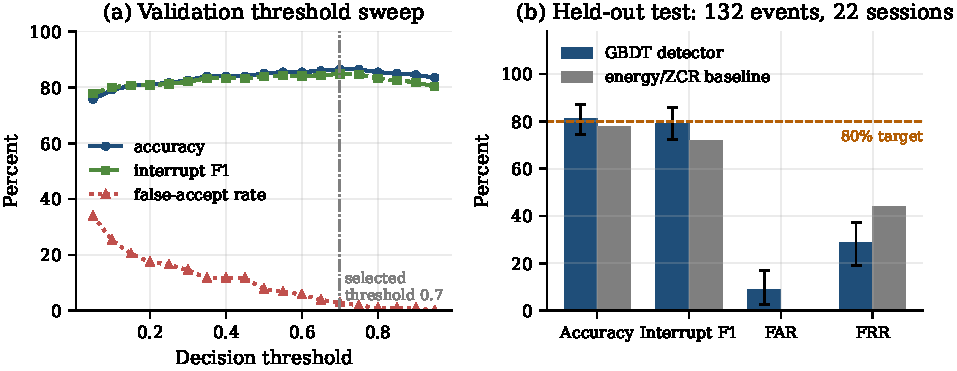
\includegraphics[width=\textwidth]{figs/bargein_proxy.pdf}
\caption{(a) Search for the decision threshold on the validation sessions; the vertical
         line is the selected threshold of 0.70. (b) Comparison of the proposed detector
         with the energy baseline on the test sessions; the error bars are session-level
         block confidence intervals.}
\label{fig:bargein}
\end{figure}

Against the baseline, the proposed detector shows a clear improvement in the F1 of the
interruption class and a marked reduction of the false reject rate. The energy baseline has
a false accept rate of zero, but at the cost of rejecting 43.94\% of real interruptions,
which in an interactive system means repeatedly ignoring the user.

\claim{The point accuracy of 81.06\% is above 80\%, but the lower bound of the session-level
block confidence interval is 74.44\% and falls below 80\%. More importantly, the reference
labels of this evaluation come from automatic speaker diarization and have no independent
human review. Requirement R5 is therefore ``not proven'' by this evidence.}

\subsection{Deployment Simulation}
\label{sec:res-bargein-sim}

The deployed controller (Section~\ref{sec:bargein}) was measured in a simulation that
reconstructs the microphone during playback of the assistant's reply: residual echo of the
reply (18--32 dB below the user and 20--60 ms later), background noise, a room response and
one real event at the start, middle or end of the reply: an interruption (real Persian
speech), a real backchannel, a real noise burst, or nothing. Six development runs used only
the audio of the training split (Table~\ref{tab:bargein-dev}), and the chosen variant was
run once on 600 scenarios of the test split (Table~\ref{tab:bargein-sim}).

\begin{table}[ht]
\centering
\caption{Development runs of the simulation (training split only)}
\label{tab:bargein-dev}
\small
\begin{tabular}{llr}
\toprule
Run & Change & Dev accuracy / F1 \\
\midrule
dev3 & duration/MLP confirm + double-talk detector & 0.687 / 0.624 \\
dev4 & lexical ASR confirm with echo rejection & 0.840 / 0.765 \\
dev5 & + coupling prior, wider echo matching, function words & 0.920 / 0.862 \\
dev6 & + one-frame duck (latency tie-break) & 0.913 / 0.856 \\
dev7 & + 200 ms confirm pre-roll (not kept) & 0.900 / 0.840 \\
\bottomrule
\end{tabular}
\end{table}

\begin{table}[ht]
\centering
\caption{One-time result of the simulation on 600 test scenarios (95\% Wilson intervals)}
\label{tab:bargein-sim}
\small
\begin{tabular}{lr}
\toprule
Measure & Value \\
\midrule
Accuracy (interrupt = positive) & \textbf{0.933} (0.910--0.951) \\
F1 & \textbf{0.880} \\
Interruptions stopped (recall) & 0.980 (0.943--0.993) \\
Stop rate: backchannel / noise / no event & 0.087 / 0.093 / 0.067 \\
Onset $\rightarrow$ duck, median / p90 & \textbf{120} / 247 ms (66\% $\le$ 150 ms) \\
Onset $\rightarrow$ stop, median / p90 & 786 / 1344 ms \\
\bottomrule
\end{tabular}
\end{table}

Accuracy and F1 are both above 0.80, and the median time to duck is 120 ms. A complete stop
takes longer (median 786 ms), because the controller waits until a word is heard; during
this interval the assistant's volume is ducked. The largest jump in the development runs
came from two places: the lexical confirmation (which separates backchannels and echo from
interruptions) and fixing the initialization of the double-talk detector's coupling
factor. The seventh run, after the evaluation, tested adding 200 ms of audio before the
onset to the input of the lexical confirmation: more interruptions were stopped (0.98
versus 0.95) but more backchannels and noise too, so by the same rule it was set aside.

\claim{This result is on simulated mixtures of real recordings, not live users; the echo is
modelled as attenuated and delayed assistant speech, and the labels come from extraction
rules and a recognizer with a list of listener tokens, not from people.}

\section{Continuity of the Full-Duplex Transport}
\label{sec:res-duplex}

The automatic regression test of the WebSocket layer passed with four tests. These tests
confirm that the 3,200-sample pre-roll before the interruption is combined with the 1,600
samples received after it to build a 4,800-sample input for the next turn. They also cover
receiving the stop acknowledgement from the client, runtime identity telemetry, turn
cancellation, concurrent connections, reconnection, isolation of session state, truncated
or silent input, recovery from generation and out-of-memory errors, and a metrics-only
retention mode that writes no audio file.

The final repository audit also recorded 206 passing tests with 65\% branch coverage
(against a required 60\%) and type checking without errors on 49 files.

\claim{This evidence proves continuity at the level of the server transport. A physical
browser run and a target-hardware run were not performed; requirement R2 therefore remains
met in software and officially unproven.}

\section{Direct Track: Seven Experimental Generations}
\label{sec:res-moshi}

\subsection{Overall Result}

Table~\ref{tab:moshi-summary} summarizes the seven experimental generations. The common
pattern of all generations is the same: the loss decreases and the autoregressive runtime
condition is not met.

\begin{table}[ht]
\centering
\caption{Summary of the seven experimental generations of the direct track. The ``best
         run'' column is the largest number of the nine rows of the runtime panel passed
         among all checkpoints of that generation.}
\label{tab:moshi-summary}
\small
\begin{tabular}{lrrrrc}
\toprule
\textbf{Version} & \textbf{Window} & \textbf{Candidates} & \textbf{Minimum} &
\textbf{Best} & \textbf{Eligible} \\
 & \textbf{(s)} & & \textbf{loss} & \textbf{run} & \\
\midrule
v1   & 20  & 16 & 1.402 & 0/9 & no \\
v2   & 100 & 20 & 1.735 & 2/9 & no \\
v3   & 100 & 5  & 1.879 & 1/9 & no \\
v4   & 100 & 5  & 1.879 & 1/9 & no \\
v5   & 100 & 5  & 1.868 & 1/9 & no \\
v6.2 & 12  & 4  & 2.060 & 0/9 & no \\
v7a  & 12  & 4  & 1.264 & 6/9 & no \\
\bottomrule
\end{tabular}
\end{table}

\claim{The minimum loss values are ``not directly comparable'' across generations, because
the text window, the validation set and the number of evaluation samples differ between
generations. For versions v6.2 and v7a the loss is computed on the training data itself and
is an in-sample measure. This column is shown only to illustrate the downward trend of the
loss within each generation.}

Figure~\ref{fig:trials} sets these two axes against each other: offline loss decreased in
every generation, but no generation reached the condition of 9 of 9.

\begin{figure}[ht]
\centering
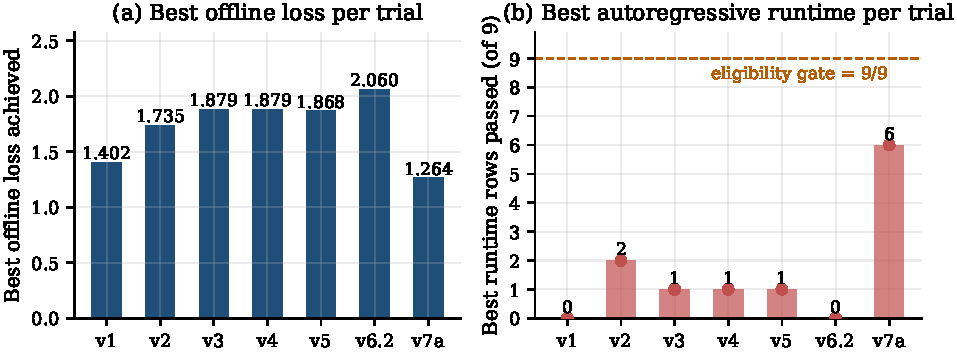
\includegraphics[width=\textwidth]{figs/moshi_trials_summary.pdf}
\caption{(a) Best offline loss of each generation. (b) Largest number of rows passing the
         nine-row runtime panel in each generation, against the acceptance condition of 9
         of 9.}
\label{fig:trials}
\end{figure}

\subsection{Version One: Positive Held-Out Loss, Failed Runtime}

Version one was trained for up to 8000 steps with a 20-second window.
Figure~\ref{fig:v1}(a) shows the training loss and part (b) the re-evaluated validation loss
of 16 checkpoints. The validation loss decreased monotonically, and the checkpoint of step
8000 with a loss of 1.402444 was selected.

\begin{figure}[ht]
\centering
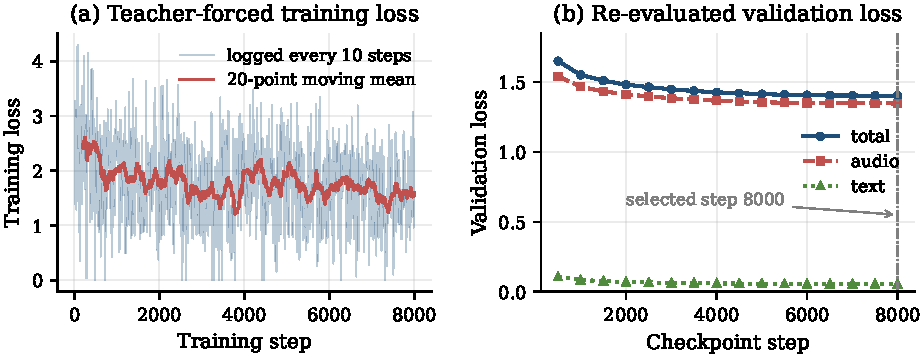
\includegraphics[width=\textwidth]{figs/moshi_v1_training.pdf}
\caption{(a) Teacher-forced training loss of version one, with a rolling mean.
         (b) Re-evaluated validation loss by text and audio component; the vertical line is
         the selected checkpoint.}
\label{fig:v1}
\end{figure}

On the held-out test set with 204 rows and 331 segments, this adapter gave a total loss of
1.7272 with a 95\% confidence interval of 1.5866--1.8678, against 3.5670 for the unadapted
base model and 9.9871 for a control group in which the sign of all $B$ matrices of the
adapter was flipped. That is, in terms of the training objective, the adapter improved
significantly over both the base model and the control. The total loss is the sum of the
mean cross-entropies of the text and audio tokens; in terms of perplexity (the exponential of
the mean loss), the perplexity of the text tokens fell from 2.53 to 1.19 and that of the
audio tokens from 13.98 to 4.71. This is the ``reduction of perplexity on a Persian test
set'' that the second objective of the proposal asks for; the second part of that objective,
``intelligible output'', was not met.

Nevertheless, the same selected adapter produced almost silent audio and no text in the
official streaming server. This contradiction is the observation that made the runtime
acceptance condition necessary for the following generations.

\subsection{Version Two: The Clearest View of the Gap}

Version two, with a 100-second text window and 20 candidate checkpoints, is the clearest
illustration of the central pattern of this project. Table~\ref{tab:v2} shows several points
of this trend and Figure~\ref{fig:v2} gives the full picture.

\begin{table}[ht]
\centering
\caption{A sample of version-two checkpoints: the validation loss decreases monotonically
         while the number of rows passing the runtime panel does not increase}
\label{tab:v2}
\small
\begin{tabular}{rrrrr}
\toprule
\textbf{Step} & \textbf{Total loss} & \textbf{Text loss} &
\textbf{Audio loss} & \textbf{Panel passes} \\
\midrule
100  & 2.312407 & 0.402789 & 1.909618 & 0/9 \\
400  & 1.894230 & 0.201763 & 1.692467 & 2/9 \\
800  & 1.792216 & 0.164635 & 1.627582 & 1/9 \\
1000 & 1.768085 & 0.155691 & 1.612394 & 1/9 \\
1500 & 1.739114 & 0.144936 & 1.594178 & 0/9 \\
2000 & 1.734574 & 0.143414 & 1.591161 & 0/9 \\
\bottomrule
\end{tabular}
\end{table}

\begin{figure}[ht]
\centering
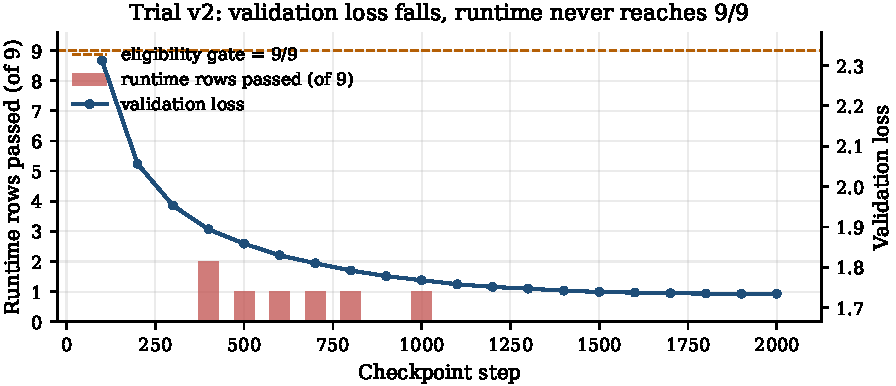
\includegraphics[width=\textwidth]{figs/moshi_v2_loss_vs_runtime.pdf}
\caption{Version two: the validation loss on 202 segments decreases monotonically over the
         checkpoints (line), while the number of rows passing the nine-row runtime panel
         (bars) never reaches the acceptance condition.}
\label{fig:v2}
\end{figure}

The decisive point is that the best runtime behaviour occurs at step 400, where the loss is
\emph{higher}, and as the loss keeps falling until step 2000, the runtime behaviour gets
\emph{worse} and reaches zero. That is, in this setting the validation loss is not even
positively correlated with generation quality.

\subsection{Versions Three to Five: Testing Targeted Hypotheses}

The next three versions tested specific hypotheses (Table~\ref{tab:moshi-design}). Version
three froze all embeddings and raised the rank to 128. Version four trained only the two text
embeddings, and version five lowered the first-codebook loss weight from 100 to 10.
Table~\ref{tab:v45} shows the row-by-row result of the last two versions.

\begin{table}[ht]
\centering
\caption{Result of each checkpoint of versions four and five on the nine-row runtime panel}
\label{tab:v45}
\small
\begin{tabular}{rrrrrrr}
\toprule
& \multicolumn{3}{c}{\textbf{Version four}} &
  \multicolumn{3}{c}{\textbf{Version five}} \\
\cmidrule(lr){2-4}\cmidrule(lr){5-7}
\textbf{Step} & \textbf{Loss} & \textbf{Speech} & \textbf{Pass} &
                \textbf{Loss} & \textbf{Speech} & \textbf{Pass} \\
\midrule
100 & 2.082125 & 9/9 & 1/9 & 2.082676 & 9/9 & 0/9 \\
200 & 1.948315 & 7/9 & 0/9 & 1.943459 & 7/9 & 0/9 \\
300 & 1.899640 & 4/9 & 0/9 & 1.889862 & 6/9 & 0/9 \\
400 & 1.881632 & 5/9 & 1/9 & 1.870719 & 5/9 & 1/9 \\
500 & 1.879061 & 5/9 & 0/9 & 1.867859 & 4/9 & 1/9 \\
\bottomrule
\end{tabular}
\end{table}

The common pattern of these two tables is notable: as the loss decreases, the number of rows
that produce \emph{any speech at all} falls from 9 to 4 or 5. That is, while the model fits
the training objective better, it leans more towards silence in autoregressive generation.
The peak allocated memory of version four was 28.640 GB.

All three versions closed ``fail-closed'' with zero eligible checkpoints, no adapter was
selected, and the firewall of the final test was never opened.

\subsection{Version Six: Separating Capacity from Generation}

Version v6.2 is an in-sample falsification test: training and evaluation on the same 32
samples. The result, as shown in Table~\ref{tab:v62} and Figure~\ref{fig:v62}, is two-sided
and clear.

\begin{table}[ht]
\centering
\caption{Version v6.2: a positive in-sample learning signal against a negative
         autoregressive runtime result}
\label{tab:v62}
\small
\begin{tabular}{rrrrc}
\toprule
\textbf{Step} & \textbf{Total loss} & \textbf{Text loss} &
\textbf{Audio loss} & \textbf{Panel passes} \\
\midrule
50  & 2.636405 & 0.812474 & 1.823931 & 0/9 \\
100 & 2.245344 & 0.638987 & 1.606357 & 0/9 \\
150 & 2.071542 & 0.550852 & 1.520690 & 0/9 \\
200 & 2.060297 & 0.551183 & 1.509114 & 0/9 \\
\bottomrule
\end{tabular}
\end{table}

\begin{figure}[ht]
\centering
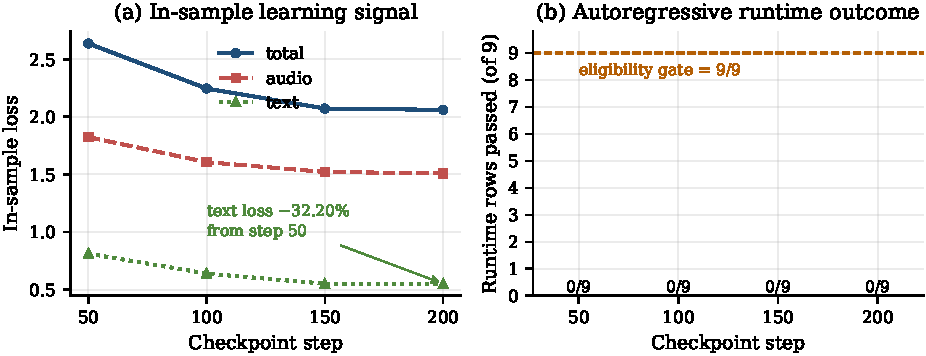
\includegraphics[width=\textwidth]{figs/moshi_v62_diagnostic.pdf}
\caption{Version v6.2: (a) the in-sample loss decreases steadily, and the text loss falls by
         32.20\% from step 50 to the best later step. (b) Nevertheless all four checkpoints
         pass 0 of the 9 rows of the runtime panel.}
\label{fig:v62}
\end{figure}

The best text loss after step 50 is 0.550852, which is 32.20\% lower than the value at step
50 (0.812474) and above the predefined criterion of 30\%. That is, this adapter has the
\emph{capacity} to fit the training objective.

At the same time, all four checkpoints pass 0 of the 9 rows of the runtime panel, and in each
checkpoint only one of the nine rows produces text and speech together. The precise
conclusion is:

\begin{quote}
Version v6.2 learned the limited in-sample training objective, but the learned behaviour did
not transfer to reliable autoregressive generation of Persian speech and text.
\end{quote}

\claim{No checkpoint of any of the first six generations is eligible for deployment, and no
final test was opened for the direct track. The statement ``Moshika was successfully
fine-tuned for Persian'' is \emph{false} on this evidence. The correct conclusion is ``a
negative experiment with a positive learning signal''.}

\subsection{Version Seven: Removing the Tokenizer Bottleneck}
\label{sec:res-moshi-v7}

Version v7a, on the same 32 samples and the same nine-row panel, showed the largest
improvement in autoregressive generation of all the Moshi experiments
(Table~\ref{tab:moshi-v7}). The in-sample teacher-forced text loss went from 1.124 at step 50
to 0.0149 at step 150, and from that step on the official server produced audible speech (RMS
about 0.07--0.19) with fluent pseudo-Persian text on 8 of the 9 rows.

\begin{table}[ht]
\centering
\caption{Number of accepted rows of the nine-row panel in the in-sample capacity test}
\label{tab:moshi-v7}
\small
\begin{tabular}{lrrrr}
\toprule
Experiment (same 32 rows) & Step 50 & Step 100 & Step 150 & Step 200 \\
\midrule
v6 (Persian script, turn-level span, sampled text) & 0/9 & 1/9 & 1/9 & 1/9 \\
v6.1 (v6 weights, greedy text; controlled baseline) & 0/9 & 0/9 & 1/9 & 3/9 \\
v6.2 (Persian script + text-input dropout) & 0/9 & 0/9 & 0/9 & 0/9 \\
\textbf{v7a (romanized phonemes + word timing)} & 0/9 & 0/9 & \textbf{6/9} & 4/9 \\
\bottomrule
\end{tabular}
\end{table}

Still, the ``all nine rows'' condition was not met: three rows of step 150 were rejected with
prefix errors of 0.76 and 0.91 (slightly above the 0.75 limit) and one row that was always
silent. The pre-registered secondary measure is negative too: the speech of step 200 has a
mean prefix error of 0.88 with the deployed recognizer, and no row reaches the 0.75 limit. By
the protocol, full training of v7b was therefore not started and the sealed test was not
opened. The result is two-sided: the tokenizer bottleneck is real, and removing it turned
almost silent output into audible speech with text, but it is not the only obstacle; despite a
near-zero teacher-forced loss, the generated text drifts from the memorized target, which is
the sign of the same gap between teacher forcing and free generation
(Section~\ref{sec:exposure-bias}).

\section{The Speech-Input Track}
\label{sec:res-speechin}

Table~\ref{tab:speechin} compares the three speech-input arms with the deployed system on 60
natural turns and 60 elderly requests (with a simulated elderly voice: two male Piper voices,
speed 0.85 and room noise).

\begin{table}[ht]
\centering
\caption{The speech-input track against the cascade (Qwen3.8-27B judge)}
\label{tab:speechin}
\small
\begin{tabular}{lrrrrr}
\toprule
Arm & Rel. nat. & Rel. eld. & Rel. all & Coh. & First token \\
\midrule
ASR $\rightarrow$ Qwen3-4B (deployed) & \textbf{2.85} & 2.75 & \textbf{2.80} & 3.36 & 86 ms \\
ASR $\rightarrow$ Gemma 4 text & 2.03 & \textbf{2.95} & 2.49 & 3.69 & 98 ms \\
Gemma 4 audio, zero-shot & 1.65 & 2.32 & 1.98 & 3.60 & \textbf{67 ms} \\
Gemma 4 audio + LoRA & 1.97 & 2.13 & 2.05 & \textbf{3.81} & 200 ms$^{*}$ \\
\bottomrule
\end{tabular}
\par\smallskip{\footnotesize $^{*}$ Serving overhead of an unmerged adapter in vLLM.}
\end{table}

The adapter lowered the held-out loss from 1.296 to 0.712, but the relevance of the best
speech arm is 0.75 below the deployed system (difference interval $-1.05$ to $-0.46$); by
the pre-registered rule the result is therefore negative, and the cascade stayed. Three
points follow from this comparison. First, removing recognition lowers quality even with the
same language model (2.49 versus 1.98); the bottleneck is Gemma's understanding of Persian
speech, not Persian text generation. Second, self-distillation on in-domain speech helps but
hurts outside the domain: on real turns, the adapter closed most of the gap to its text
teacher (1.65 to 1.97, teacher 2.03), but on the requests with a synthetic voice it got worse
(2.32 to 2.13). Third, the time saving is negligible, because CTC recognition adds only about
20 ms to the time to first token.

With the second judge (Gemini), the picture is reversed: the deployed system gets the lowest
relevance (1.91), text Gemma with the elderly prompt 3.00, and the speech path 2.18 zero-shot
and 2.52 with the adapter. The decision rule was registered with the first judge and the
official result stays negative, but this disagreement is the same disagreement of the two
judges about the deployed responder. Under both judges, removing recognition lowers quality.
The larger Gemma~4~12B does not understand Persian speech better either: its speech path is
weaker than E4B under both judges (1.48 and 1.63), while its text mode is better.

\section{Latency, Memory and Browser Loopback}
\label{sec:res-latency}

The final system was measured with the automated loopback test of Section 6.4 of the
proposal: a headless Chromium browser opens the real client page with a fake microphone that
plays recorded Persian utterances of 1--5 seconds, and the audio travels the same path as a
real user's. Times were measured with the client's clock: from the frame holding the acoustic
end of speech to the scheduled start of the first clause of the reply. The protocol was
registered before running, and every planned turn (even an unanswered one) is in the
denominator.

\textbf{Memory.} Requirement R6 is a 12--24 GB GPU, and such hardware was not available; this
deviation is declared. To measure the ``fit'', the language model server was limited to a
0.105 share of the H100's memory, so that the GPU side of the whole system fits in a 12 GiB
card (12,288 MiB). The peak measured in the final run was \textbf{11,336~MiB} (11.1~GiB):
9,730~MiB reserved by the language model and 1,606~MiB for recognition (10,994~MiB in the first
run); the synthesizer and the voice activity detector run on the CPU. The compute speed,
however, is the H100's.

\textbf{Two runs.} The first run (v1) used a speculative start after 160 ms of silence. Because
the first clause was ready about 390 ms after the end of speech, that is, much later than the
confirmation of the end of the turn (256 ms), starting the speculative work earlier lowers
latency without changing when a turn is confirmed or cut. Under a pre-registered protocol,
values of 64, 96, 128 and 160 ms were measured on 60 development utterances that were in no
test panel, and the rule chose 96 ms (audible 90th-percentile latency 488 versus 541 ms for
the previous value). The second run (v2) measured the same test panels again with this value;
this is a second measurement of the same panels and is reported as such
(Table~\ref{tab:latency}).

\begin{table}[ht]
\centering
\caption{Latency from end of speech to the assistant's first audio in the browser loopback test
         (ms). Main panel: 61 PSRB utterances and 140 corpus utterances; elderly: the same
         method with speed 0.85 and 3 dB quieter; barge-in: the base turns of the two
         interruption panels. The last column adds the browser's reported output latency.}
\label{tab:latency}
\small
\begin{tabular}{llrrrrrrr}
\toprule
Panel & Run & Turns & Mean & Median & p90 & Max & $\le$500 ms & Audible p90 \\
\midrule
Plain & v1 & 201 & 418 & 415 & 487 & 537 & 93.5\% & 529 \\
 & \textbf{v2} & 201 & \textbf{372} & 375 & \textbf{431} & \textbf{491} & \textbf{100\%} & \textbf{473} \\
Elderly & v1 & 80 & 435 & 433 & 508 & 575 & 86.3\% & 550 \\
 & \textbf{v2} & 80 & \textbf{382} & 371 & \textbf{446} & 546 & 98.8\% & 488 \\
Barge-in & v1 & 120 & 399 & 388 & 464 & 509 & 99.2\% & 506 \\
 & \textbf{v2} & 120 & \textbf{366} & 363 & \textbf{415} & 497 & 100\% & 457 \\
\bottomrule
\end{tabular}
\end{table}

In the final run no turn went unanswered, and the mean (372) and 90th percentile (431) of the
main panel are below 500 ms; the strict reading ``every turn below 500 ms'' is also met for the
main panel (maximum 491). Adding the browser's reported output latency (about 42 ms), the 90th
percentile is 473 and 98\% of turns are below 500 ms. The 90th percentile for simulated elderly
speech is 446 ms, and only one turn of 80 exceeded 500 ms. The stage shares (medians, from the
speculative start): recognition 65, first token 42 ms after that, completion of the first clause
85 and its audio 56 ms, plus the 96 ms of silence before the speculative start.

\textbf{Interruptions in a real browser.} In 60 turns with a real interruption and 60 turns with
a real backchannel (selected with an independent recognizer), 47 interruptions were stopped and
8 backchannels were stopped by mistake: accuracy \textbf{0.825} and F1 \textbf{0.817} (first
run 50 interruptions and the same 8 wrong stops: 0.850 and 0.847; a difference of three events
in 60 is within sampling variation). The median time to duck from the detected onset frame was
44 ms (90th percentile 60) and the median time to stop 507 ms; the time from the real acoustic
onset in the simulation was 120 ms (Section~\ref{sec:res-bargein-sim}).

\textbf{The reply after an interruption.} The proposal asks for interruptions to be simulated
at the start, middle and end of the reply and for the coherence of the new reply to be
measured. In 30 scripted dialogues, an elderly request and then a dependent follow-up question
(such as \textpersian{«صبر کن، من زانوم درد می‌کنه، باز هم پیاده‌روی کنم؟»}, meaning ``wait, my knee hurts,
should I still go walking?'') were played in a synthesized user voice: once over the
assistant's reply (0.8, 1.8 or 3.0 seconds after the end of the request) and once as a normal
turn after the reply had ended. Of the 27 interruptions that arrived during playback, 24
stopped the reply (start and middle 10 of 10, end 4 of 7). The two automatic judges rated the
reply to the follow-up question equally in both conditions: relevance 1.67 against 1.67 under
Gemini and 2.90 against 2.80 under Qwen, with the same use of the context of the first request;
the pre-registered criterion (a drop of at most 0.25) was therefore met. The absolute level of
the scores is the level of the responder itself. In the first run of this test, the
synthesizer's pauses inside the user's sentences made end-of-speech detection close the
requests prematurely; that run was not scored, and the sentences were synthesized again
without internal pauses (this phenomenon also occurs in real speech;
Section~\ref{sec:res-errors}).

\textbf{Semantic end-of-turn detection (tested twice and rejected).} To reduce premature closing of
a turn at mid-sentence pauses, a pre-registered ``gate'' was tested: at the speculative start,
a model estimates the probability that the utterance is complete, and if it is low,
confirmation of the end of the turn is postponed until 640 or 1024 ms of silence. Three
zero-shot candidates (Smart Turn v3.2~\cite{smartturn2025}, which does not support Persian, a
completeness judgement of the transcript by the same Qwen3-4B, and a rule on words such as
\fa{«که»} and \fa{«را»} with which a Persian utterance cannot end) and a version of Smart Turn
fine-tuned on Persian speech were measured on 850 development trials (425 podcast utterances
from sessions outside the test panels, plain and simulated elderly) with an exact replay of the
end-of-speech detector. Without a gate, 19.8\% of trials are closed prematurely. All candidates
reduced this (the best zero-shot candidate to 13.3\%), but none met the condition ``delaying at
most 5\% of genuine ends'' (lowest 13.1\%, the lexical rule). Some of these delays are correct,
because many of the development utterances are cut mid-sentence; but zero-shot Smart Turn is
close to chance on Persian, and Persian data with natural turn endings were scarce (738
training examples). The first fine-tuned model was declared invalid because of a data artifact
(the audio was cut at the moment of the speaker change), and the protocol was amended before the
corrected run. No gate qualified in this first round.

A second pre-registered round fixed both data problems. Each development clip's ending was
labelled by Gemini in two independent passes (158 complete, 224 unfinished and 43 uncertain
endings), and false holds were counted only on complete endings. Smart Turn was also
fine-tuned again on 5,498 examples mined from 233 hours of restored diarized windows (the
label filter was cut short when the shared Gemini budget ran out). With correct holds no
longer counted, the Qwen3-4B completeness judgement ($\theta = 0.3$, hold 640 ms) met the
development rule: premature closings fell from 19.8\% to 13.3\% while 4.4\% of complete
endings were held. The retrained Smart Turn still held 29\% or more. The gate then went to
the loopback test, whose panels were opened for the first time. It split fewer utterances
than before (17 against 22 over both panels, not significant), but it also held 44 finished
turns (14.8\%), and each hold delayed the reply by up to 384 ms. The 90th percentile of the
latency rose to 656 ms on both panels, above the 500 ms limit, so the pre-registered rule
removed the gate and the deployed detector stayed unchanged.

\claim{This automated loopback test is on the shared H100 host: the memory of a 12 GB card was
respected but not its speed, and there was no human user and no physical microphone and
loudspeaker path (and therefore no acoustic echo). This is not the target-hardware condition of
the proposal.}

\section{Error Analysis}
\label{sec:res-errors}

The proposal asks for the failure modes to be classified. Table~\ref{tab:errors} puts the
failures of each stage side by side, from the receipts of this chapter.

\begin{table}[ht]
\centering
\caption{Failure modes of the system and the measured cause of each}
\label{tab:errors}
\small
\begin{tabular}{L{3.2cm}L{3.5cm}L{6.4cm}}
\toprule
\textbf{Failure mode} & \textbf{Frequency} & \textbf{Measured cause} \\
\midrule
Latency above 500 ms & 0 of 201 main turns and 1 of 80 elderly turns (first run: 13 and 11) &
  in the slow turns, the stage furthest above its median was ``completion of the first
  clause'', that is, token generation stalls on the shared GPU; neither recognition nor
  synthesis \\
Missed interruption & 13 of 60 in the browser; 2\% in simulation &
  4 times there was no duck (no frame louder than the expected echo); 9 times it ducked but
  the confirmation transcript had no content word and the reply continued \\
Premature turn end mid-sentence & 15 of 201 main and 7 of 80 elderly utterances &
  a mid-sentence pause longer than the 256 ms end-of-turn confirmation; when the user goes on,
  the system stops the reply and keeps both fragments in the history, but the first,
  incomplete reply starts; a semantic end-of-turn gate was tested and rejected \\
Wrong stop on a backchannel & 8 of 60 in the browser; 8.7\% in simulation &
  the recognizer heard a listener token as a content word; an observed example:
  \fa{«آره آره»} as \fa{«کار»} (first phoneme clipped) \\
Recognition error & character error 9.44\%; older speakers 15.6\% &
  the speech of older adults (consistent with the literature, Section~\ref{sec:elderly-lit});
  a word error rate much higher than the character error rate because of spelling variation and
  joined writing (Section~\ref{sec:disc-cer-wer}) \\
Irrelevant or weak reply & Gemini judge: 2.38 of 4 &
  the two automatic judges disagree about the responder's quality; only human judging is
  conclusive \\
Unintelligible synthesized speech & character error 5.82\% (Mana) &
  residual pronunciation errors of the synthesizer; in the lab VITS model, the ezafe and
  suffixes after a ZWNJ \\
Unintelligible direct-track speech & prefix error 0.88 (v7a) &
  the tokenizer bottleneck and the gap between teacher forcing and free generation
  (Section~\ref{sec:res-moshi}) \\
\bottomrule
\end{tabular}
\end{table}

\section{Human Study}
\label{sec:res-study}

The instrument of the small listening study is a self-contained Persian page that runs without
recording audio and without asking for a name: consent and age group, naturalness scores (1 to
5) for 8 sentences in the Mana voice, the same 8 sentences in the ganji\_adabi voice, 6 samples
of natural human speech as anchors and an attention check, and then three recorded dialogues
with the live system (a question and answer, a backchannel in the middle of a reply, and an
interruption with a new question), with scores for response speed, reaction to the
interruption, satisfaction and willingness to use. To arbitrate between the two automatic judges
of the responder, eight elderly requests are shown with two replies (the deployed system and
Qwen3.5-4B with the elderly prompt) in random order, and the participant picks the better reply.
By a rule registered before the study was sent, the deployed responder changes to Qwen3.5-4B
only if participants prefer its replies (the confidence interval of the preference difference
above zero, and no participant over 60 picking the deployed reply more often) and this same
configuration passes the deployment qualification (memory, latency, coherence after
interruption). The protocol and the method of analysis were registered before sending.

The results of this study had not yet been received when this version was written.

\claim{Until the participants' responses arrive, no claim is made about the naturalness of the
speech or the experience of older adults.}

\section{The Latency, Size and Quality Trade-off}
\label{sec:res-tradeoff}

Table~\ref{tab:tradeoff} puts all measured candidates of each component side by side with their
size, quality and latency (Question 3 of the proposal). The parameter counts were taken from the
model files themselves.

\begin{table}[ht]
\centering
\caption{The size, quality and latency trade-off of the candidates (quality and latency from the
         tests of the previous sections)}
\label{tab:tradeoff}
\small
\setlength{\tabcolsep}{4.5pt}
\begin{tabular}{llrlr}
\toprule
Stage & Candidate & Params & Quality & Latency \\
\midrule
ASR & NeMo v4 CTC (deployed) & 117M & CER 9.44\% & 58 ms \\
 & Shenava Koochik & 115M & CER 8.95\% & 65 ms \\
 & omniASR CTC 1B & 976M & CER 14.04\% & 56 ms \\
 & Rade-ASR-CTC-3B (Persian) & 3.08B & CER 16.11\% & 122 ms \\
 & Seamless v5 fine-tune & 1.50B & \textbf{CER 6.92\%} & 671 ms \\
 & Whisper large-v3 & 1.54B & CER 23.02\% & 1101 ms \\
 & Qwen3-ASR 1.7B & 2.35B & CER 20.47\% & 1466 ms \\
 & Gemma 4 E4B (audio input) & 8.61B$^{a}$ & CER 21.04\% & 2632 ms \\
\midrule
Responder$^{b}$ & Qwen3-4B, prompt-v2 (deployed) & 4.02B & 2.80 / 1.91 & 86 ms \\
 & Gemma 4 E4B, elderly prompt & 8.61B$^{a}$ & 2.49 / 3.00 & 98 ms \\
Speech input$^{b}$ & Gemma 4 E4B, audio in & 8.61B$^{a}$ & 1.98 / 2.18 & 67 ms \\
 & + speech LoRA & 8.61B$^{a}$ & 2.05 / 2.52 & 200 ms \\
Responder$^{d}$ & Qwen3.5-4B, elderly prompt & 4.66B & 3.23 / 3.35 & 68 ms \\
 & four larger models & 9.65--36.0B & 2.77--3.24 / 3.48--3.61 & 53--121 ms \\
\midrule
TTS & Piper Mana (deployed, CPU) & 15.7M & \textbf{CER 5.82\%} & 84 ms \\
 & Lab VITS, optimized (H100) & 36.3M & CER 9.19\% & 116 ms \\
 & ParsVoice-XTTS (H100) & -- & CER 13.55\% & 1751 ms \\
\midrule
Direct S2S & Moshika LoRA (v7a) & 7.69B & unintelligible$^{c}$ & -- \\
\bottomrule
\end{tabular}
\par\smallskip\footnotesize
$^{a}$ Stored parameter count; the model name refers to about 4 billion ``effective''
parameters.
$^{b}$ Relevance of the reply to the same 120 spoken turns; the first number is the Qwen judge
and the second the Gemini judge; latency is the first token after the end of the audio.
$^{c}$ Prefix error 0.88 with the deployed recognizer.
$^{d}$ Relevance on the 120 written requests and turns of Table~\ref{tab:resp-size}, Qwen
judge / Gemini judge, under a 22~GiB limit; latency is the first token of the reply text.
Gemma~4 31B did not fit.
\end{table}

Three patterns appear. First, within this range size does not buy quality. The two smallest
recognizers (115 and 117 million parameters, both NeMo models fine-tuned on Persian) are more
accurate than every larger candidate except Seamless. That includes Rade, a
three-billion-parameter model fine-tuned on Persian. Seamless, the only model more accurate
than them, is itself fine-tuned on Persian and more than ten times slower. In synthesis too, the
smallest model (Piper, 15.7 million parameters) is both the most intelligible and the fastest.
Second, for the responder and speech input, the two judges disagree about quality. No larger
candidate is better under both judges, up to 36 billion parameters at four bits
(Table~\ref{tab:resp-size}), and the largest dense model at four bits does not fit a 22~GiB
limit. The speech-input model has only a latency advantage (67 versus 86 ms), which separate
recognition in about 60 ms can make up for. Third, the largest
model, the 7.7-billion-parameter end-to-end model, did not reach intelligible Persian speech with
low-cost training. For real-time Persian with these resources, the best trade-off point is small
components specialized for Persian.

\section{Final Status of the Requirements}
\label{sec:res-requirements}

Table~\ref{tab:req-status} sets the status of each of the seven requirements of
Table~\ref{tab:requirements} against the evidence obtained.

\begin{table}[ht]
\centering
\caption{Final status of the seven requirements of the project definition and the class of the
         supporting evidence}
\label{tab:req-status}
\small
\begin{tabular}{cL{4.2cm}L{6.2cm}}
\toprule
\textbf{ID} & \textbf{Status} & \textbf{Supporting evidence} \\
\midrule
R1 & met (streaming cascade) &
     40-row final semantic test; all 401 loopback turns were answered \\
R2 & met in loopback and simulation &
     interruption accuracy/F1 0.83/0.82 in the browser and 0.93/0.88 in simulation \\
R3 & met by the proposal's criterion and, on the main panel, by the every-turn reading &
     mean 372 and 90th percentile 431 ms; all turns below 500; with the browser's output latency a 90th percentile of 473 \\
R4 & met &
     108.584 hours of audited export (automatic labels) \\
R5 & accuracy goal met by another method &
     two-stage controller with lexical confirmation; energy/pitch/MFCC classifier alone 0.574 \\
R6 & declared deviation &
     whole-system memory measured at 11.1~GiB; speed on an H100 \\
R7 & awaiting results &
     registered instrument and protocol; results not yet available \\
\bottomrule
\end{tabular}
\end{table}

\claim{The evidence for R2, R3 and R5 is automated (browser loopback and simulation from real
recordings) and on an H100, not a human test or target hardware. R4 has no human labels. R5 was
not met by the acoustic features specified in the project definition alone; lexical
confirmation with the speech recognizer replaced them.}

Of the four expected outputs of the project definition, three have been produced and documented:
a working prototype for the cascade track, documented source code with an open licence and an
automated test suite, and the Persian conversational dataset. For the fourth item, the
listening-study instrument and its method of analysis are registered; empirical findings on older
adults can be reported only once the participants' responses arrive.
